\chapter{Redesign Strategy}
\label{chapter:redesignstrategy}
Several weaknesses and flaws of the web view of AMCS have been identified and analyzed in the previous chapter. They range from issues regarding visualization, layout and space usage to problems with user navigation.
A set of proposals that aim at solving these problems is introduced in the subsequent chapter. The focus will predominantly lie on using the available screen space more efficiently, improving local navigation inside polls and global navigation between different views and reducing indirection to a minimum.
\begin{wrapfigure}{l}{0.5\textwidth}
	\vspace*{-0.5cm}
	\begin{center}
		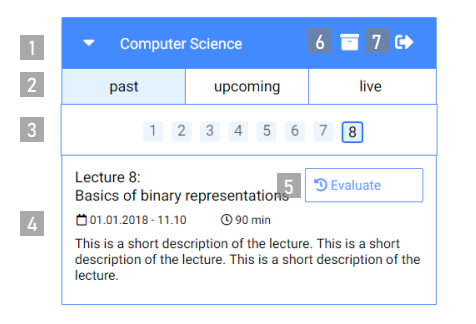
\includegraphics[width=0.48\textwidth]{mockups/main_view_enhancement_v1_annotated.png}
	\end{center}
	\captionsetup{format=plain}
	\caption{Mock-up 1 of the new \emph{Main View}: Currently, the \emph{past courses} tab is shown.
		A course that has already taken place is selected.
		Usage of drop down menus and tabs to reduce the amount of vertical space used. (5), (6) and (7) serve as buttons to evaluate given answers for the shown lecture, go to the question pool of this course and unsubscribe from the selected course respectively.
	}
	\label{figure:mainviewenhancement}
	\vspace*{-1.5cm}
\end{wrapfigure}
Each proposal for itself is centered around improving usability aspects of the application while all proposals as a whole aim at keeping the interface consistent and recognizable across all supported platforms.
As already mentioned in \Cref{chapter:stateoftheart}, AMCS was extended in a modular fashion over the years. This resulted in UI components that each differ in varying degrees from each other visually. 
No redesign of all modular components is attempted, but rather a redesign of the overall framework in which these components are embedded, narrowing down the focus of this work even further.
\section{Main View}
Several improvements for the layout and visualization of the \emph{Main View} are elaborated in this section. \Cref{figure:mainviewenhancement}, \Cref{figure:mainviewenhancement2} and \Cref{figure:mainviewenhancement3} respectively show an evolution of mock-ups for the \emph{Main View}.
\subsection{Layout}
\label{section:con:proposals:mainview:layout}
\paragraph{Iteration 1}
As mentioned in \Cref{section:con:problems:mainview:generalvis}, the \emph{Main View} suffers from using the available vertical space not effectively enough. Most noticeably, the course overview and \emph{Enrollment Form} are placed below the \emph{Lecture List}. In order to find information about relevant courses or to enroll in or leave a course, students are required to scroll all the way to the bottom. 
Therefore, one proposal is to compress this view by using drop-down menus and tabs.  \Cref{figure:mainviewenhancement} represents a mock-up of the proposals described in the following. 
First of all, the view is restructured to follow the hierarchical concept of courses containing lectures: In the top (1), a button for a drop-down menu is shown next to the currently selected courses' name and two additional buttons (6) and (7). The purpose of the drop-down menu and the buttons is explained later.
Following the heading, tabs for \emph{past}, \emph{upcoming} and \emph{live} lectures are laid out side-by-side (2). In the first two mock-ups (see \Cref{figure:mainviewenhancement} and \Cref{figure:mainviewenhancement2} respectively), the tabs are followed by the \emph{Navigation Bar}, a numbered horizontal list of clickable dots (3) that each represent one lecture. The currently selected lecture is highlighted with a bold blue border to enhance visibility and orientation. Finally, the information section of the view follows (4) with the title of the lecture, time and duration details and the lecture description. In the details section, an additional button is placed (5) that is labeled as “Evaluate”.
\begin{wrapfigure}{r}{0.5\textwidth}
	\vspace*{-0.5cm}
	\begin{center}
		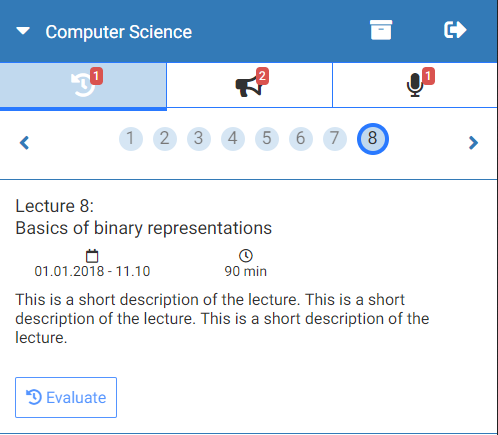
\includegraphics[width=.48\textwidth]{mockups/main_view_enhancement_v2_cropped.png}
	\end{center}
	\captionsetup{format=plain}
	\caption{Mock-up 2 of the new \emph{Main View}:
		Textual descriptions for tabs are replaced with iconography, notification
		bubbles for unread content are introduced. Colors are adjusted to match the corporate design of AMCS.
	}
	\label{figure:mainviewenhancement2}
	\vspace*{-0.5cm}
\end{wrapfigure}
Another idea would be to hide or deactivate this button for lectures that have not yet entered the state \emph{past}. This layout uses a considerably reduced amount of vertical space.
The placement of the “Evaluate” button (5) is motivated by reducing vertically occupied space even further. However, it could be reasonable to place it below the description text of the lecture. On most devices, the proposed layout will reduce the amount of scrolling required. In an effort to keep visual clutter and redundancy at a minimum, the badges that indicate temporal context of the lectures now miss completely.
The view will solely rely on the sorting of lectures in their respective tabs, meaning that the tabs themselves visually convey the temporal context of a lecture.
\paragraph{Iteration 2}
After collecting feedback from the AMCS group, the mock-up was adjusted slightly (see \Cref{figure:mainviewenhancement2}). The textual description of the tabs is replaced with iconography. Furthermore, \emph{Notification Bubbles} are introduced to indicate new or unread content. The \emph{Evaluate Button} was moved to a more conventional location at the bottom of the view. The number of simultaneously displayed lectures remains at one.
\paragraph{Iteration 3}
Regarding the strict reduction of vertical space used by the layout, one might suggest that the new \emph{Main View} has become too compact.
Feedback from the AMCS group led to the realization, that multiple lectures should be visible at the same time for the reason that typically multiple lectures are taking place on the same day.
Therefore, the next iteration expands the layout again to display three lectures at once (see \Cref{figure:mainviewenhancement3}). A page view concept is proposed that tries to find a compromise between minimizing scrolling and maximizing the amount of information displayed at once. The location of the \emph{Evaluate Button} is moved again to the top portion of a lecture box.
\subsection{Navigation}
\label{section:con:proposals:mainview:navigation}
Tabs (2) will separate lectures by their temporal context. Selecting a tab will only display lectures that share the respective temporal context, meaning that it should be easier to switch between \emph{past}, \emph{upcoming} and \emph{live} lectures.
The \emph{Navigation Bar} (3) in \Cref{figure:mainviewenhancement3} is used to ease navigation between lecturesthat share the same temporal context. A student can use the bar to switch quickly between the oldest and newest past lecture by selecting the corresponding
\begin{wrapfigure}{l}{0.5\textwidth}
	\vspace*{-0.5cm}
	\begin{center}
		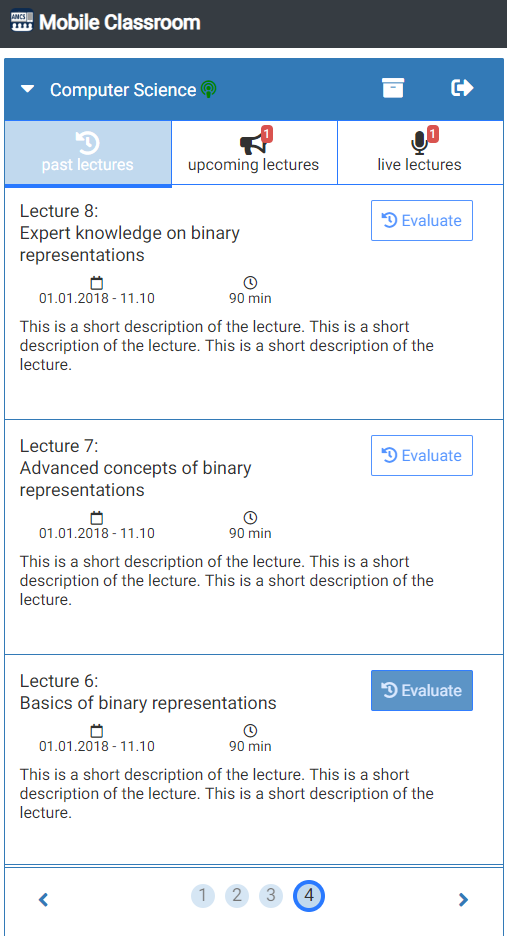
\includegraphics[width=0.48\textwidth]{mockups/main_view_enhancement_v3.png}
	\end{center}
	\captionsetup{format=plain}
	\caption{Mock-up 3 of the new \emph{Main View}:The icon indicating an ongoing lecture for a course is brought back.A combination of textual description and iconography is used for tabs.Multiple lectures are displayed at once in a page-based view.}
	\label{figure:mainviewenhancement3}
	\vspace*{-0.5cm}
\end{wrapfigure} button from the bar. This should improve navigation within the \emph{Main View} as well as in the context of a lecture.  Additionally, this proposal aims at removing indirection in the global navigation context by providing certain buttons that serve as shortcuts for the functionality currently found in the \emph{Burger Menu}. Button (6) serves as a shortcut to the \emph{Question Pool} for the selected course. On click of button (7), the student will be removed from the selected course. Both of these buttons are placed in the header of the layout next to the course’s name to indicate that both referenced functionalities operate in the context of courses, whereas the “Evaluate” button (5) operates on the context of lectures.
\newline
\newline 
As previously described in \Cref{sec:soa:eval_of_answers}, the \emph{Evaluation of Answers} requires the user to select a course and a lecture of interest from two drop-down menus.
The \emph{Evaluate Button} will eliminate the need to select both the course and lecture of interest. The information required for the back-end request that returns the answers for a given lecture is present. The idea is therefore to reuse the existing \emph{Evaluation of Answers} component, but have the click on the \emph{Evaluate Button} select the course and lecture for the user. This way, two extra steps are removed from the established workflow.
All three buttons try to reduce the indirection introduced by the \emph{Burger Menu} to a minimum. Features associated with a course or lecture will be accessible from a view that deals with courses or lectures respectively. The \emph{Burger Menu} will then only have to deal with the profile editing and logout functionalities.

\subsection{Drop-Down Menu}
\label{section:con:proposals:dropdown}
The \emph{Drop-Down Menu} is introduced to help reducing usage of vertical space even more (see \Cref{figure:embeddeddropdown}). Clicking on it reveals its two functions: Besides the now embedded \emph{Enrollment Form}, a list of courses a student is already enrolled to is shown below.
When selecting a course from this list, only corresponding lectures will be shown in the \emph{Main View}.
The \emph{Enrollment Form} still consists of a text field and a button. Both elements are shown next to the text \emph{Enroll...}. The close proximity to the list of courses could make the \emph{Enrollment Form} potentially more traceable to users. The \emph{Enrollment Form} will only be embedded in the drop down menu when the student is enrolled in at least one course beforehand. Otherwise, if a student has not enrolled in any course yet, in place of the \emph{Main View}, only the \emph{Enrollment Form} will be shown.
In summary, the \emph{Drop Down Menu} acts as a coarse grain filter to the \emph{Main View} and essentially covers the responsibilities of the \emph{Course View} that is currently in place.
\begin{wrapfigure}{r}{0.5\textwidth}
	\begin{center}
		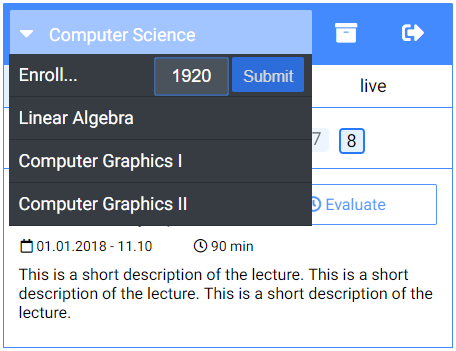
\includegraphics[width=.48\textwidth]{mockups/embedded_drop_down.png}
	\end{center}
	\captionsetup{format=plain}
	\caption{Mock-up of the new \emph{Embedded Drop Down Menu}:
		The enrollment form is integrated in the menu. Users can change the currently selected course from here. The \emph{Main View} then adapts accordingly, allowing the menu to act as a filter for courses.
	}
	\label{figure:embeddeddropdown}
	\vspace*{-0.75cm}
\end{wrapfigure}

\section{Poll View}
\label{section:con:proposals:pollview}

\subsection{Layout and Visualization}
Several issues have been identified regarding layout and visualization of polls in \Cref{section:con:problems:pollview}. Main problems include the ineffective use of vertical space and a lack of visual separation between poll types. Regardless of their type, polls are simply appended to the bottom of the list.
The view therefore grows unnecessarily in size. In order to solve these issues, a tab-based layout is proposed once more. \Cref{figure:pollviewenhanvement1} shows the first mock-up iteration for the redesign of the \emph{Poll View}.
\paragraph{Iteration 1}
Beginning at the top, the course's name is displayed in white font on a blue rectangle (1). Following up, to separate the type of polls from one another, a \emph{Tab Menu} is used (2) to differentiate between \emph{Slide Polls}, \emph{Lecture Polls} and \emph{Course Polls}. The tabs are arranged from left to right depending on the poll's lifetime. The most short lived polls, the \emph{Slide Polls} are placed on the left, the \emph{Lecture Polls} take advantage of the middle and the \emph{Course Polls} are displayed to the right. Selecting one of the tabs will cause the layout to show only polls of said type, making them act as a filter to what is currently displayed. This will potentially improve the effectiveness of vertical space used significantly. 

\begin{figure}[ht]
	\begin{minipage}[t]{\textwidth}
		\centering
		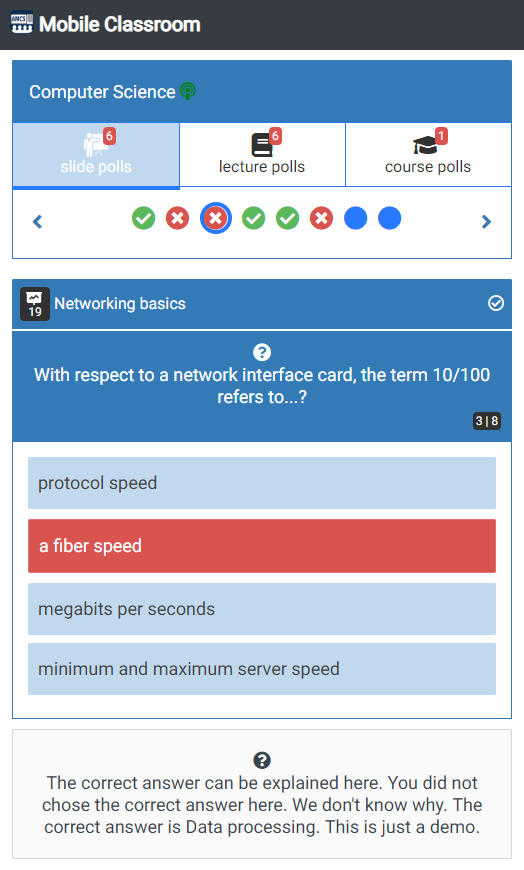
\includegraphics[width=.7\textwidth]{mockups/poll_view_enhancement_v2.png}
		\captionsetup{width=.8\linewidth}
		\caption{Mock-up 2 of the new \emph{Poll View}:
			Colors are adapted to match the corporate design of AMCS.
		}
		\label{figure:pollviewenhanvement2}
	\end{minipage}
\end{figure}
Below the \emph{Tabs}, a \emph{Navigation Bar} (3) is displayed that contains the question's topic, index and the total number of questions. In case of a slide poll, the current slide number is shown additionally (see \Cref{figure:pollviewenhanvement1}).
Furthermore, the \emph{Navigation Bar} introduced in \Cref{section:con:proposals:mainview:navigation} is reused here (4). It serves as a means to navigate between questions more easily and faster. However, the \emph{Navigation Bar} also reduces vertical space used significantly. Only one question at a time is displayed to the student.
\newline
\newline
Appropriate colors and icons are intended to convey information more efficiently. A blue bold border is used to indicate the current question selected in the \emph{Navigation Bar}, light blue dots signify, that the corresponding question has not been answered yet, whereas bold green or red dots indicate correctly and wrongly answered questions respectively. 
Below the \emph{Navigation Bar}, only one question at a time is displayed to the student to avoid visual noise and clutter (5). The question is displayed in a blue rectangle with white text. Below the question, an instance of an answering mechanism is displayed (6). 
Currently, each questions is answered individually by selecting the option and then pressing the blue \emph{Answer} button (see \Cref{figure:pollview}). Afterwards, feedback is shown immediately to the student. In terms of usability, users might find this tedious and redundant. One idea that comes to mind is to send the answers of a poll collectively in bulk to the server at the end of a poll. An advantage with this approach is the reduced amount of requests sent to the server. However, AMCS follows a rather strict principle of providing immediate feedback.
\begin{wrapfigure}{l}{0.5\textwidth}
	\begin{center}
		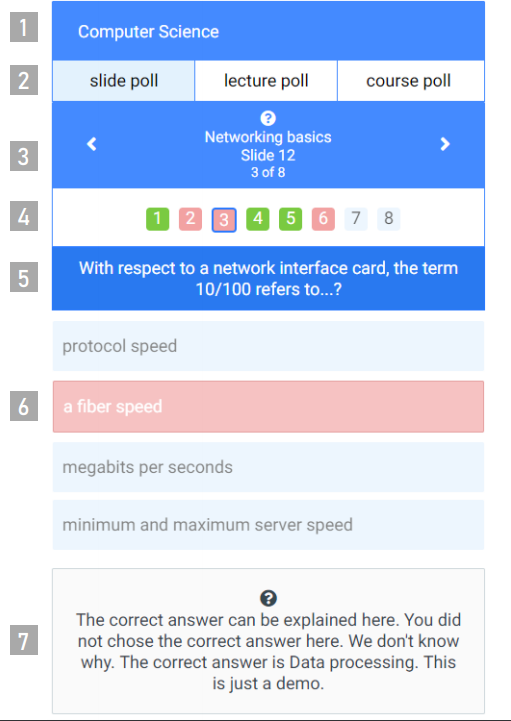
\includegraphics[width=.48\textwidth]{mockups/poll_view_enhancement.png}
	\end{center}
	\captionsetup{format=plain}
	\caption{Mock-up 1 of the new \emph{Poll View}:
		The icon indicating an ongoing lecture for a course is brought back.
		A combination of textual description and iconography is used for tabs.
		Multiple lectures are displayed at once in a page-based view.
	}
	\label{figure:pollviewenhanvement1}
	\vspace*{-0.75cm}
\end{wrapfigure}
Students should directly be informed about a the correctness of an answer.
Therefore, in the case of SC-, MC-, SCC- or MCC-questions, the button to answer the question is omitted and merely selecting an option will trigger a request to the back end server.
Wrong answers are highlighted as before in red, a correct answer in green and it will still be possible to answer twice. Finally, space for textual feedback is given in a box (7) below the answers. This view is reusable and can therefore also be used to display already answered questions when using the \emph{Evaluate answers} functionality. This view will likewise profit from the reduced amount of vertical space used. 
\paragraph{Iteration 2}
Similar to the later iterations of the \emph{Main View} described earlier, the mock-up was adapted to comply with the corporate design of AMCS (see \Cref{figure:pollviewenhanvement2}).
The tabs at the top now use textual descriptions and iconography simultaneously to convey their meaning more efficiently, as feedback by the AMCS group led to the assumption that icons alone are not recognizable enough. The tabs are further enhanced by the inclusion of \emph{Notification Bubbles} that indicate the amount of unanswered question in each poll category, potentially reducing the cognitive effort to find unanswered questions.
The \emph{Navigation Bar} is further enhanced by using icons that represent the state of a specific question. Green arrows and red crosses are used to visualize correctly or wrongly answered questions respectively to improve accessibility, especially for colorblind students.
In order to separate navigation from content, the buttons that allow to jump between questions are moved to the \emph{Navigation Bar}, as they resided previously next to the topic and question.
The indicator for the current slide number is modified slightly and pushed to the left. On the right side, the icons that differentiate between question types are reintroduced. 
\subsection{Navigation between questions}

Navigation between questions should be made easier for students and focus on one question at a time. Therefore, an improvement would be to introduce two buttons in the \emph{Navigation Bar} that can be used to navigate one question forward or backwards. Pressing the respective button will cause to show the next or previous question, regardless of whether the current question has already been answered. This leads to the same level of freedom when navigating polls that the current state of the application allows.
\newline
\newline
Swiping is a widely spread way of interacting with a user interface on smartphones or tablets. Consequently, a student might expect to be able to use these gestures while using AMCS. Therefore, navigating between questions should be possible by swiping left to go forward or right to go backwards. The combination of swiping and the provision of buttons for navigation enhances usability while respecting different platforms and device types. Students on smartphones and tablets will have buttons and swipe gestures simultaneously available to them, while users on laptops and computers without touchscreens can use the buttons.
In addition to that, the student can use the indicators inside the \emph{Navigation Bar} to freely select a question they wish to answer or review. This eases navigation within a poll and only very little scrolling is required if any at all.


\section{Course View}
The \emph{Course View} has an important function in terms of usability. It acts as a filtered view on all lectures belonging to a certain course. Users will seek the opportunity to sort and filter lectures, which is why this function must be replicated by the redesign. However, as described in \Cref{section:con:problems:courseview}, the \emph{Course View} has a redundant nature as it looks and feels nearly identical to the \emph{Main View}.
Furthermore, some potentially confusing click paths lead to the \emph{Course View} as elaborated in \Cref{section:con:problems:navigation}.
As outlined in \Cref{section:con:proposals:dropdown}, the \emph{Drop-Down Menu} filter lectures after a course they belong to. The tabs below allow for additional filtering after the temporal context of lectures. 

Therefore, with these proposals in place, the \emph{Course View} is deemed obsolete. Dropping the \emph{Course View} from the redesign results in shorter, fewer click paths and stronger interconnectedness between all views (see \todogrf{Add graphic of new click paths}).

\subsection{Navigation}
By shifting navigation elements from the old \emph{Burger Menu} to components of the \emph{Main View}, the new \emph{Burger Menu} is slimmed down.
It only contains the buttons labeled \emph{How it works}, \emph{Edit account} and \emph{Login/Logout}. The options to view the \emph{Question Pool}, to \emph{Evaluate} a given lecture or to unsubscribe from a course are all moved to the \emph{Main View}, as described in  \Cref{section:con:proposals:mainview:layout} and \Cref{section:con:proposals:dropdown}.
These changes lead to shorter click paths with well-defined behavior (see \todogrf).

\section{Summary}
All proposals and their respective goals are shortly summarized in \Cref{tab:proposals}. It serves as a reference to which features have to be implemented by the prototype. Therefore, this table will be referenced in \Cref{chapter:implementation}.

\cleardoublepage
\renewcommand*{\arraystretch}{1.5}
\begin{small}
	\begin{longtable}{ p{0.7cm} p{3.8cm} p{1cm} p{6.6cm}}
		\hline
		ID & Name & Views & Goals \\ \hline
		MV1 & Lecture Tabs & \emph{MV}& 
		\vspace{-0.45cm}
		\begin{itemize}[leftmargin=*, noitemsep, topsep=0pt,  partopsep=0pt]
			\item[$\cdot$] Visual separation of lectures
			\item[$\cdot$] Filter lectures by temporal context
			\item[$\cdot$] Reduce amount of vertical space used
		\end{itemize} \vspace{-0.45cm} \\ 
		MV2 & Drop Down Menu & \emph{MV} & 
		\vspace{-0.45cm}
		\begin{itemize}[leftmargin=*, noitemsep, topsep=0pt]
			\item[$\cdot$] Filter lectures by course
			\item[$\cdot$] Reduce amount of vertical space used
		\end{itemize} \vspace{-0.45cm} \\ 
		MV3 & Embedded Enrollment Form &\emph{MV} &
		\vspace{-0.45cm}
		\begin{itemize}[leftmargin=*, noitemsep, topsep=0pt]
			\item[$\cdot$] Reduce cognitive effort to enroll to a course
			\item[$\cdot$] Reduce amount of vertical space used
		\end{itemize} \vspace{-0.45cm} \\ 
		MV4 & Improved Lecture Visualization &\emph{MV} &
		\vspace{-0.45cm}	
		\begin{itemize}[leftmargin=*, noitemsep, topsep=0pt]
			\item[$\cdot$] Reduce cognitive effort to find information
			\item[$\cdot$] Reduce visual clutter
			\item[$\cdot$] Reduce amount of vertical space used
		\end{itemize} \vspace{-0.45cm} \\ 
		MV5 & Improved Location of Access To Features &\emph{MV} &
		\vspace{-0.45cm}	
		\begin{itemize}[leftmargin=*, noitemsep, topsep=0pt]
			\item[$\cdot$] Reduce amount of vertical space used
			\item[$\cdot$] Reduce click path length
			\item[$\cdot$] Remove unnecessary click paths
		\end{itemize} \vspace{-0.45cm} \\ 
		MV6 & Pagination Of Lectures &\emph{MV} & 
		\vspace{-0.45cm}	
		\begin{itemize}[leftmargin=*, noitemsep, topsep=0pt]
			\item[$\cdot$] Reduce amount of vertical space used
			\item[$\cdot$] Reduce visual clutter
			\item[$\cdot$] Remove unnecessary click paths
		\end{itemize} \vspace{-0.45cm} \\ 
		PV1 & Poll Tabs & \emph{PV} &
		\vspace{-0.45cm}	
		\begin{itemize}[leftmargin=*, noitemsep, topsep=0pt]
			\item[$\cdot$] Reduce amount of vertical space used
			\item[$\cdot$] Reduce visual clutter
		\end{itemize} \vspace{-0.45cm} \\ 
		PV2 & Improved Visualization of Questions & \emph{PV} &
		\vspace{-0.45cm}	
		\begin{itemize}[leftmargin=*, noitemsep, topsep=0pt]
			\item[$\cdot$] Improve visuals and readability
			\item[$\cdot$] Reduce visual clutter
		\end{itemize} \vspace{-0.45cm} \\ 
		PV3 & Navigation Bar & \emph{PV} &
		\vspace{-0.45cm}	
		\begin{itemize}[leftmargin=*, noitemsep, topsep=0pt]
			\item[$\cdot$] Improve navigation between questions
			\item[$\cdot$] Reduce visual clutter
			\item[$\cdot$] Reduce amount of vertical space used
		\end{itemize} \vspace{-0.45cm} \\
		PV4 & Next/Back Buttons & \emph{PV} &
		\begin{itemize}[leftmargin=*, noitemsep, topsep=0pt]
			\item[$\cdot$] Improve navigation between questions
		\end{itemize} \vspace{-0.45cm} \\ 
		PV5 & Support Swiping & \emph{PV} &
		\vspace{-0.45cm}	
		\begin{itemize}[leftmargin=*, noitemsep, topsep=0pt]
			\item[$\cdot$] Improve navigation between questions
			\item[$\cdot$] Improve quality of user interaction
		\end{itemize} \vspace{-0.45cm} \\ 
		NV1 & Slimmed Down Burger Menu & \emph{BM} & 		\vspace{-0.45cm}	
		\begin{itemize}[leftmargin=*, noitemsep, topsep=0pt]
			\item[$\cdot$] Improve global navigation
			\item[$\cdot$] Reduce click paths and their length
			\item[$\cdot$] Reduce amount of vertical space used
		\end{itemize} \vspace{-0.45cm} \\ 
		NB & Notification Bubbles & \emph{MV}, \newline \emph{PV} &
		\vspace{-0.45cm}	
		\begin{itemize}[leftmargin=*, noitemsep, topsep=0pt]
			\item[$\cdot$] Improve quality of user interaction
			\item[$\cdot$] Reduce cognitive effort to find new content
		\end{itemize} \vspace{-0.45cm} \\ \hline
		\caption{Classification of proposals for improved usability of AMCS. This classification serves as a feature list for the prototype. MV = Main View, PV = Poll View, BM = Burger Menu}
		\label{tab:proposals}
	\end{longtable}
\end{small}
